\chapter{Artificial Neural Networks}

\section{Theory}
Artificial Neural Networks (ANN) also called multilayer perceptron, can be used as a model for pattern recognition. 
In    
\begin{figure}[H]
\centering
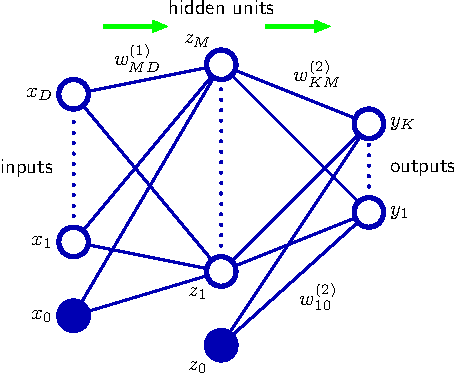
\includegraphics{Figure5_1}
\caption{Results of using ANN with 3 speakers, 30 hidden variables and 1 digit spoken}
\label{fig:ANN_fig_theory}
\end{figure}

\section{Method}



\section{Result}


\subsection{Single digit:}
\begin{figure}[H]
\centering
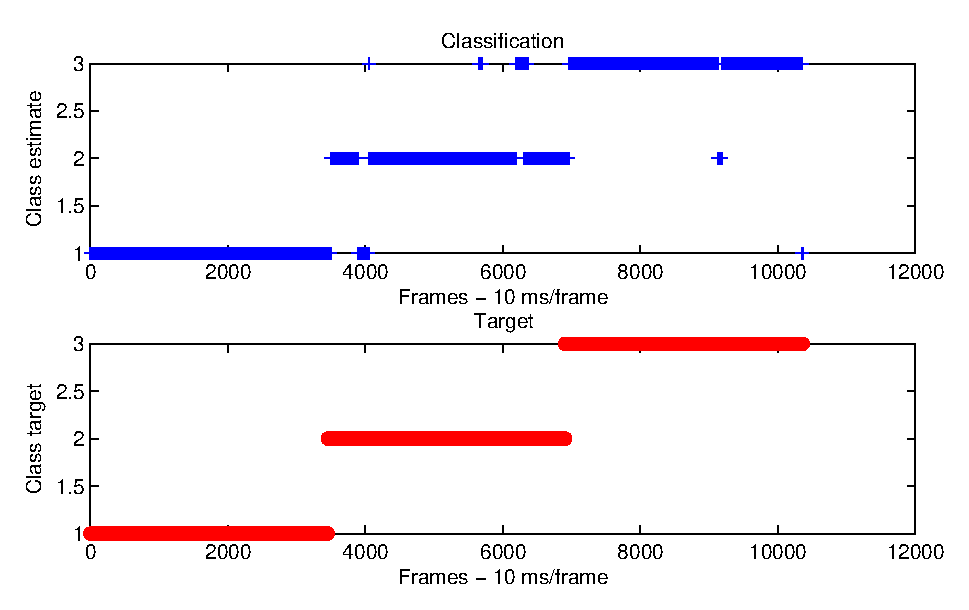
\includegraphics{ANN_1digit_8cent_3speak}
\caption{Results of using ANN with 3 speakers, 30 hidden variables and 1 digit spoken}
\label{fig:ANN_fig_1}
\end{figure}

\begin{table}[H]                                                    
\centering                                                          
\begin{tabular}{|l|c|c|c|c|}                                        
\hline                                                              
  & Speaker Jacob & Speaker Mose & Speaker Simon & Precision [\%] \\
\hline                                                              
Estimate Jacob & 3454.0 & 196.0 & 11.0 & 94.3 \\                    
\hline                                                              
Estimate Mose & 0.0 & 3077.0 & 104.0 & 96.7 \\                      
\hline                                                              
Estimate Simon & 0.0 & 181.0 & 3339.0 & 94.9 \\                     
\hline                                                              
Sensitivity [\%] & 100.0 & 89.1 & 96.7 & 95.3 \\                    
\hline                                                              
\end{tabular}                                                       
\caption{Confusion matrix - 1 digit}                                
\label{table:ANN_conf_1}                                            
\end{table}  



\subsection{Two digits:}
\begin{figure}[H]
\centering
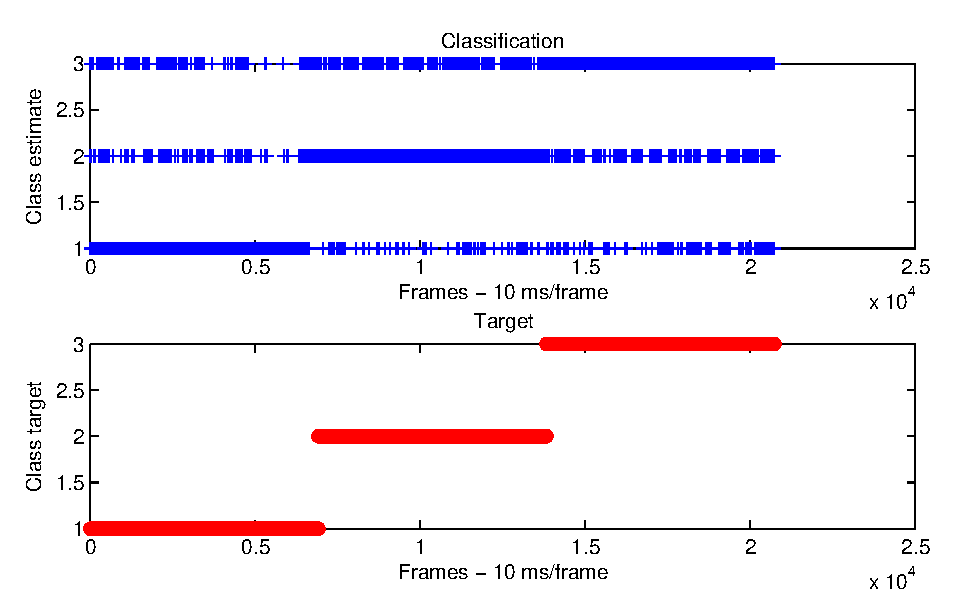
\includegraphics{ANN_2digit_8cent_3speak}
\caption{Results of using ANN with 3 speakers, 30 hidden variables and 2 digits spoken}
\label{fig:ANN_fig_2}
\end{figure}

\begin{table}[H]                                                    
\centering                                                          
\begin{tabular}{|l|c|c|c|c|}                                        
\hline                                                              
  & Speaker Jacob & Speaker Mose & Speaker Simon & Precision [\%] \\
\hline                                                              
Estimate Jacob & 6486.0 & 0.0 & 93.0 & 98.6 \\                      
\hline                                                              
Estimate Mose & 276.0 & 6485.0 & 492.0 & 89.4 \\                    
\hline                                                              
Estimate Simon & 148.0 & 425.0 & 6325.0 & 91.7 \\                   
\hline                                                              
Sensitivity [\%] & 93.9 & 93.8 & 91.5 & 93.1 \\                     
\hline                                                              
\end{tabular}                                                       
\caption{Confusion matrix - 2 digits}                               
\label{table:ANN_conf_2}                                            
\end{table}



%\subsection{Ten digits:}
%\begin{figure}[H]
%\centering
%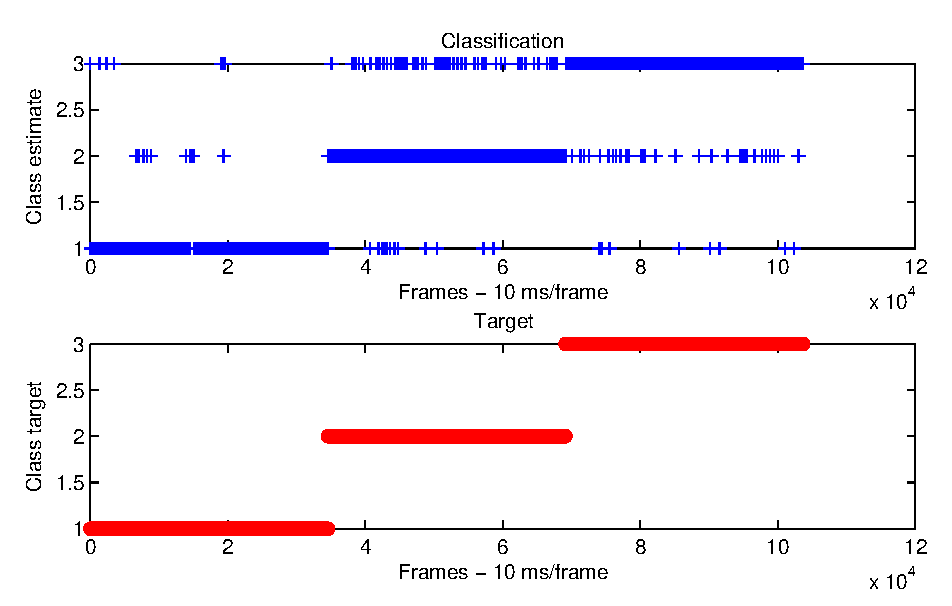
\includegraphics{ANN_10digit_8cent_3speak}
%\caption{Results of using ANN with 3 speakers, 30 hidden variables and 10 digits spoken}
%\label{fig:ANN_fig_10}
%\end{figure}
